\documentclass{article}
\usepackage[utf8]{inputenc}
\usepackage[a4paper, total={19cm, 28cm}]{geometry}
\usepackage{verbatim}
\usepackage{graphicx}
\usepackage{listings}

\title{Projeto 3: Decaimento radioativo e números aleatórios}
\author{Pedro de Carvalho Braga Ilídio Silva - 9762595}
\date{Maio de 2017}

\begin{document}
\maketitle

\section{Introdução}
As aproximações para cálculo diferencial estão presentes em quase todo computador atualmente. Elas são indispensáveis para automatizar os processos de integração e derivação, pois oferecem, com a desvantagem da imprecisão, algoritmos simples para realizar tais operações. O vigente projeto busca explirar essas características, demonstrando como desenvolver métodos computacionais para a resolução de problemas no âmbito do cálculo numérico.

\section{Derivada numérica}

Neste programa, criou-se  funções FORTRAN para calcular derivadas numéricas da função matemática $f(x)=e^{2x}\sin{x}$. Cada função FORTRAN levava dois argumentos: $x$ e $h$; e retornava o resultado de uma das fórmulas a seguir:

\begin{itemize}
\item Derivada frontal de 2 pontos: \(f_f'(x)={f(x+h)-f(x) \over h}\)
\item Derivada traseira de 2 pontos: \(f_t'(x)={f(x)-f(x-h) \over h}\)
\item Derivada simétrica de 3 pontos: \(f_{3s}'(x)={f(x+h)-f(x-h) \over 2h}\)
\item Derivada simétrica de 5 pontos: \(f_{5s}'(x)={\frac {-f(x+2h)+8f(x+h)-8f(x-h)+f(x-2h)}{12h}}\)
\item Derivada segunda simétrica de 3 pontos: \(f_{3s}''(x)=\frac{f(x+h)-2\,f(x)+f(x-h)}{h^2}\)
\item Derivada segunda simétrica de 5 pontos: \(f_{5s}''(x) ={ -f (x - 2h) + 16f (x - h) - 30f (x) + 16f (x + h) - f (x + 2h)\over 12h^2}\)
\end{itemize}

Todos as variáveis deste programa foram criadas com dupla precisão.
Organizou-se os valores retornados pelas funções criadas, para $x = 1$ e diferentes valores de $h$, nas tabelas \ref{tab:1} e \ref{tab:2}.

\begin{table}[h]
  \centering
   \begin{center}
\begin{tabular}{|c|c | c| c|}
\hline
 h & $f_f\prime(1)t$ & $(1)3s$  & $(1)5s $ & \\
 \hline
  0.50000000000000000      &   11.207415470347506      &   6.5987515078152654      &   2.3043319812661203      \\ \hline
   1.8271447853259204      &   1.6394300989379982      &   9.3857343193960219E-002 \\ \hline
   4.9999997019767761E-002 &  0.88930595119027700      &  0.84235443167722401      &   2.3475759756525605E-002 \\ \hline
  0.17405297640479489      &  0.17217462468203237      &   9.3917586137948206E-004 \\ \hline
   5.0000003539025784E-003 &   8.6790886449236382E-002 &   8.6321296162594763E-002 &   2.3479514332080953E-004 \\ \hline
   1.7320557386330648E-002 &   1.7301773746819293E-002 &   9.3918197556774885E-006 \\ \hline
   4.9999996554106474E-004 &   8.6579289144559368E-003 &   8.6532330057096374E-003 &   2.3479543713733619E-006 \\ \hline
   1.7312101392477075E-003 &   1.7310223068029984E-003 &   9.3916220578194043E-008 \\ \hline
   4.9999998736893758E-005 &   8.6558159740590668E-004 &   8.6553462118033053E-004 &   2.3488112788072613E-008 \\ \hline
   1.7311252892326934E-004 &   1.7311070768855075E-004 &   9.1061735929542920E-010 \\ \hline
   4.9999998736893758E-006 &   8.6556253474867617E-005 &   8.6555764511331290E-005 &   2.4448354452033527E-010 \\ \hline
   1.7311242917372738E-005 &   1.7311728324642672E-005 &   2.4270363496725622E-010 \\ \hline
   4.9999999873762135E-007 &   8.6568323744984355E-006 &   8.6555414249289697E-006 &   6.4547478473286901E-010 \\ \hline
   1.7300684369558894E-006 &   1.7338273607947485E-006 &   1.8794636957863986E-009 \\ \hline
   5.0000000584304871E-008 &   8.7741716114919655E-007 &   8.6341252014676684E-007 &   7.0023205012148537E-009 \\ \hline
   2.4552577571057554E-007 &   1.9856343769220075E-007 &   2.3481170785544236E-008 \\ \hline
  \end{tabular}
\end{center}

  \caption{Derivadas numéricas de $f(x)$ no ponto $x = 1$ por meio de diferentes aproximações em função do passo h.}
  \label{tab:1}
\end{table}

\begin{table}[h]
  \centering
  \input{tab2.txt}
  \caption{Derivadas numéricas de $f (x)$ no ponto $x = 1$ por meio de diferentes aproximações em função do passo h.}
  \label{tab:2}
\end{table}

Em seguida, por meio de métodos não computacionais, chegou-se à real fórmula para a derivada de f(x):
\[f'(x)=e^{2x}(2\sin{x}+\cos{x})\]
e para sua derivada segunda:
\[f''(x)=e^{2x}(3\sin{x}+4\cos{x})\]

Criou-se, a partir dessas últimas duas fórmulas, funções em FORTRAN para calcular o real valor das derivadas de $f(x)$, fazendo uso das funções nativas DEXP, DSIN e DCOS. Os valores reais das derivadas para $x=1$ e diferentes valores de $h$ foram comparados com os retornados pelas funções numéricas, sendo suas diferenças absolutas $|\epsilon|$ apresentadas pelas tabelas \ref{tab:3} e \ref{tab:4}.


\begin{table}[h]
  \centering
  \input{tab3.txt}
  \caption{Valor absoluto dos desvios em relação aos resultados exatos das derivadas numéricas de $f (x)$ no ponto $x = 1$ obtidas por meio de diferentes aproximações em função do passo h.}
  \label{tab:3}
\end{table}

\begin{table}[h]
  \centering
  \input{tab4.txt}
  \caption{Valor absoluto dos desvios em relação aos resultados exatos das derivadas numéricas de $f(x)$ no ponto $x = 1$ obtidas por meio de diferentes aproximações em função do passo h.}
  \label{tab:4}
\end{table}

Observa-se inicialmente que, conforme se diminui $h$, a precisão da aproximação aumenta: os valores das duas primeiras tabelas tendem aos valores esperados para $f'(1)$, 16.427676673177210, e $f''(1)$, 34.622325130868994; ao passo que $|\epsilon|$ mostra-se cada vez menor nas tabelas \ref{tab:3} e \ref{tab:4}.\par
Contudo, após atingir máxima precisão em algum valor de h diferente em cada caso, vê-se que acuidade dos valores começa a se perder, fato que se torna claro pelo posterior aumento de  $|\epsilon|$ nas duas últimas tabelas apresentadas. % A célula que porta os valores ótimos de $f'(1)$ ou $f''(1)$ em cada coluna destaca-se em amarelo, bem como os menores valores de $|\epsilon|$.\par
Os valores ótimos de $h$, que geraram menor desvio das aproximações, obtidos pela análise das tabelas criadas então são:

\begin{itemize}
\item $f_f'$ e \(f_t'\): Como o posterior aumento de $|\epsilon|$ após queda inicial não foi observado nesses casos, não é possível saber ao certo se o valor de $h$ que gerou o mínimo desvio é, de fato, o valor ótimo. Operações com h menores devem ser realizadas para se determinar isso.
\item \(f_{3s}'\): 9.9999999999999995E-007 e 4.9999999999999998E-007 geraram ambos o mesmo valor de $|\epsilon|$, o menor obtido.
\item \(f_{5s}'\): 1.0000000000000000E-003
\item \(f_{3s}''\):1.0000000000000000E-004
\item \(f_{5s}''\):1.0000000000000000E-003
\end{itemize}

O comportamento constatado de $|\epsilon|$ é facilmente observado ao plotar-se $\log10{|\epsilon|}$ em função do $\log10{h}$ (Gráfico 1). Percebe-se que quanto maior a  ordem de aproximação, embora sejam atingidos valores mais baixos para o desvio, maior é o $h$ ótimo (abscissa do ponto mínimo de cada série no gráfico 1). Isto se deve ao fato de que $|\epsilon|$ diminui com dependência maior de $h$ quanto maior for a ordem de aproximação. Desta forma, enquanto $h$ diminui, as aproximações de ordem mais elevada mais rapidamente atingem um valor de $|\epsilon|$ não suportado pela precisão utilizada, divergindo.


\begin{figure}[h!]
  \centering
  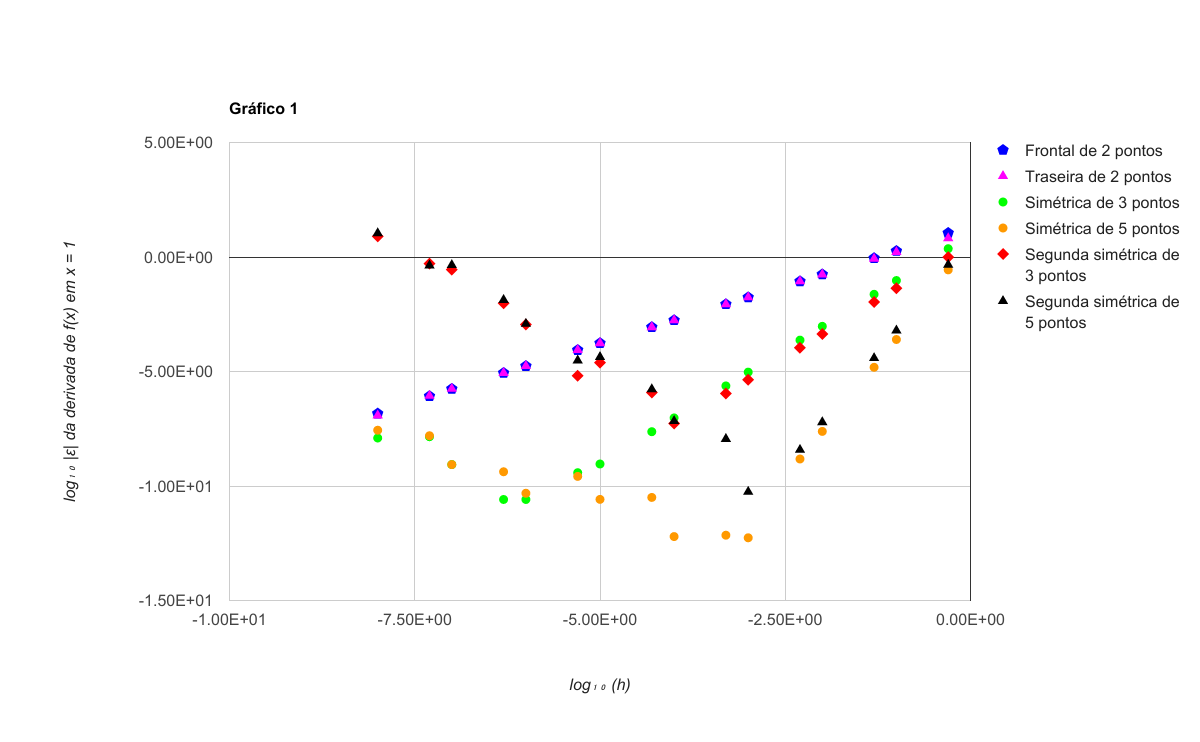
\includegraphics[width=\textwidth]{graf1}
  \caption{$log_{10}|\epsilon|$ das derivadas numéricas de $f (x)$ no ponto $x = 1$, obtidas
por meio de diferentes aproximações, em função de $log_{10}h$.}
\label{fig:1}
\end{figure}

Foram calculados somente os coeficientes de regressão linear do erro associado às derivadas de 2 pontos, pois no caso das demais, os problemas associados à precisão (aumento inesperado de $|\epsilon|$) impediriam que se constatasse a real ordem das aproximações. Para ambos os casos em que isso foi possível, obteve-se valor próximo de 1 para os coeficientes, exatamente como esperado de uma aproximação de primeira ordem e como mostrado no gráfico.

\section{Integração numérica}
Foram elaboradas duas funções FORTRAN de precisão dupla, TRAP e SIMP, para aplicar, respectivamente os métodos do Trapézio

\[\int_{a}^{b}f(x)dx \approx h [0.5f (a) + f (a + h) + f (a + 2h) + f (a + 3h) + . . . + f (b - h) + 0.5f (b)]\]

 e de Simpson

\[\int_{a}^{b}f(x)dx \approx \frac{h}{3}[f (a) + 4f (a + h) + 2f (a + 2h) + 4f (a + 3h) + 2f (a + 4h). . . + f (b)]\]

para cálculo de integrais numéricas no intervalo $[0,1]$ à função $f(x) = e^{2x}\cos{x/4}$.\par

\begin{lstlisting}
  REAL*8  FUNCTION F(X)
    REAL*8 X
    F = DEXP(2*X)*DCOS(X/4.D0)
    RETURN
  END FUNCTION F
  
  REAL*8  FUNCTION TRAP(H)
    REAL*8 H
    
    TRAP=0.
    DO I=1, 1/H-1
       TRAP = TRAP + F(I*H)
    END DO
    
    TRAP = H * (TRAP + 0.5D0 * (F(0.0D0) + F(1.D0)))
    RETURN
  END FUNCTION TRAP
  
  REAL*8  FUNCTION SIMP(H)
    REAL*8 H
    
    SIMP=0.
    DO I=1, 1/H-1
       SIMP = SIMP + (3+(-1)**(I+1)) *F(I*H)
    END DO
    
    SIMP = H/3.D0 * (SIMP + (F(0.0D0) + F(1.D0)))
    RETURN
  END FUNCTION SIMP

\end{lstlisting}

Retornos para diferentes valores de $h$ das funções acima foram comparados ao valor real da integral (3.14479185512583..., com número de casas correspondente aos 8 bytes disponíveis). Os valores absolutos para o desvio ($|\epsilon|$) são compilados pela tabela \ref{tab:5}.
\begin{table}[h]
  \centering
  \begin{tabular}{|c|c|c|}
\hline
$h$ & TRAP & SIMP \\
\hline\hline
$2^{-1}$ & 2.43581649151307E-01 & 1.31481107485722E-02 \\
\hline
$2^{-2}$ & 6.15554143340575E-02 & 8.80002728306905E-04 \\
\hline
$2^{-3}$ & 1.54308320420377E-02 & 5.59712780314747E-05 \\
\hline
$2^{-4}$ & 3.86034323131934E-03 & 3.51362774608787E-06 \\
\hline
$2^{-5}$ & 9.65250690605046E-04 & 2.19843700133282E-07 \\
\hline
$2^{-6}$ & 2.41322980663039E-04 & 1.37440157033097E-08 \\
\hline
$2^{-7}$ & 6.03313894593782E-05 & 8.59058157942627E-10 \\
\hline
$2^{-8}$ & 1.50828876330777E-05 & 5.36890532032430E-11 \\
\hline
$2^{-9}$ & 3.77072442159231E-06 & 3.35509398041722E-12 \\
\hline
$2^{-10}$ & 9.42681266380418E-07 & 2.09610107049229E-13 \\
\hline
$2^{-11}$ & 2.35670328585513E-07 & 2.08721928629529E-14 \\
\hline
$2^{-12}$ & 5.89175819243337E-08 & 2.22044604925031E-15 \\
\hline
$2^{-13}$ & 1.47294012542431E-08 & 3.10862446895043E-15\\
\hline
\end{tabular}

  \caption{Integral numérica de $f(x)$ no intervalo $[0, 1]$ por meio de duas diferentes aproximações como função da partição do intervalo $h$.}
  \label{tab:5}
\end{table}

E plotou-se $log_{10}|\epsilon|$ versus $log_{10}h$ para avaliar o comportamento do desvio (Gráfico 2).

\begin{figure}[h!]
  \centering
  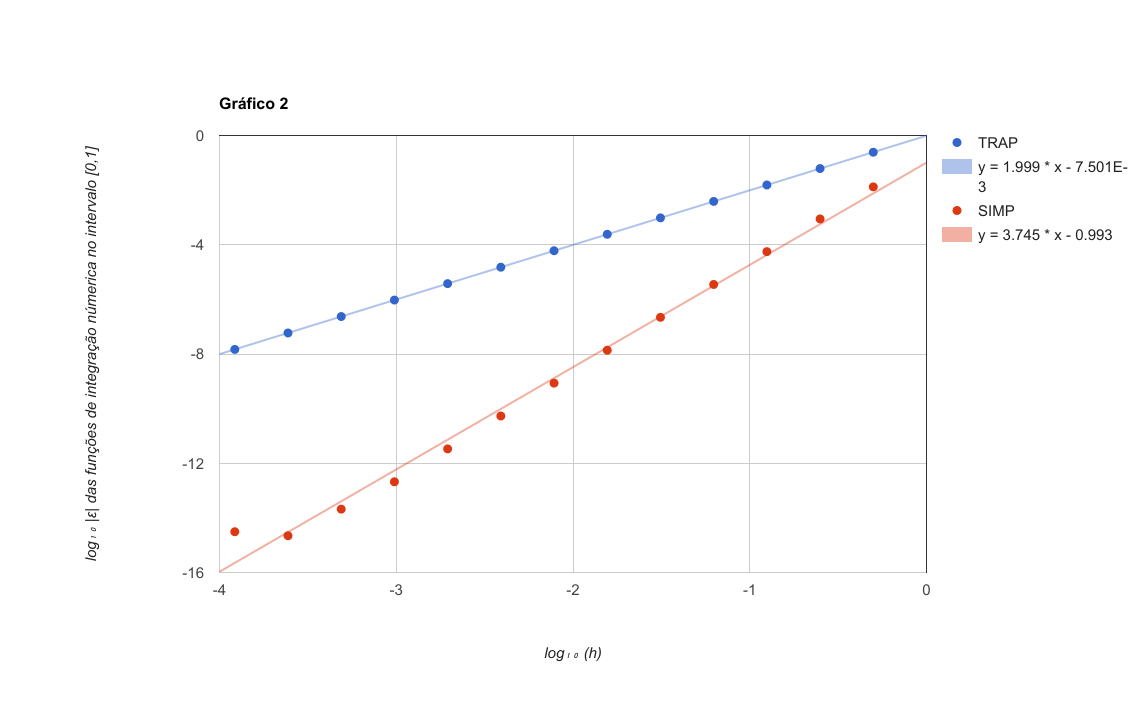
\includegraphics[width=\textwidth]{graf2}
  \caption{Integral numérica de $f(x)$ no intervalo $[0, 1]$ por meio das aproximações do Trapézio (TRAP) e de Simpson (SIMP) como função da partição do intervalo $h$.}
  \label{fig:2}
\end{figure}

Para os valores de $h$ utilizados, não se observou perda de precisão da aproximação pelo método dos trapézios à medida que $h$ diminuia, de forma que o valor mínimo de $h$ ($2^{-13}$) gerou o valor mínimo de $|\epsilon|$. Disto decorre que o não é possível afirmar que $h$ será o valor ótimo da aproximação para todo $h$ nas vigentes condições de precisão, já que valores menores de $h$ não foram testados.\par

No que se refere ao segundo caso, a aproximação de Simpson, observa-se claramente pelo gráfico que o último valor contrapôs a tendência de descida dos demais pontos. A isto se atrbui a causa da falta de precisão necessária, de forma que o valor ótimo de $h$ para as condições de precisão utilizadas foi $2^{-12}$ .\par

A regressão linear revelou ordem de convergência muito próxima de 2 para a aproximação dos Trapézios, de fato como esperado, e aproximadamente 3.735 para o método de Simpson, para o qual esperava-se obter 4.
O desvio, como claramente visto pelo Gráfico 2, se deve à não acuidade do valor da aproximação em $h = 2^{13}$, devido aos problemas de alocamento de memória insuficiente.\par
A correção das adversidades encontradas deve se basear na utilização de mais espaço de memória para as quantias com as quais se trabalhou (pelo menos 16 bytes em vez de 8) e a utilização de mais valores de $h$ para determinar mais precisamente seu valor ótimo.

\end{document}